\documentclass[aspectratio=169,12pt]{beamer}
\usepackage[T1]{fontenc}
\usepackage{lmodern}
\usepackage{amsmath,amssymb}
\usepackage{graphicx}
\usepackage{tikz}
\usetikzlibrary{arrows.meta,positioning}
\usefonttheme[onlymath]{serif}
\definecolor{Navy}{HTML}{12263A}
\definecolor{Teal}{HTML}{246B94}
\definecolor{Green}{HTML}{27815F}
\definecolor{Orange}{HTML}{B56A32}
\definecolor{Muted}{HTML}{617080}
\definecolor{Rule}{HTML}{DFE7ED}
\setbeamercolor{normal text}{fg=Navy,bg=white}
\setbeamercolor{frametitle}{fg=Navy,bg=white}
\setbeamercolor{structure}{fg=Teal}
\setbeamercolor{itemize item}{fg=Teal}
\setbeamerfont{frametitle}{size=\fontsize{18}{22}\selectfont,series=\bfseries}
\setbeamerfont{normal text}{size=\fontsize{13}{18}\selectfont}
\setbeamersize{text margin left=.8cm,text margin right=.8cm}
\setbeamertemplate{navigation symbols}{}
\setbeamertemplate{headline}{}
\setbeamertemplate{frametitle}{\vspace{.25cm}\insertframetitle\par\vspace{.12cm}}
\setbeamertemplate{footline}{%
  \hspace{.8cm}{\color{Rule}\rule{14.4cm}{.35pt}}\par
  \vspace{.08cm}
  \hfill{\color{Muted}\fontsize{8}{10}\selectfont\insertframenumber/\inserttotalframenumber}\hspace{.8cm}\vspace{.17cm}}
\setbeamertemplate{itemize items}[circle]
\setbeameroption{hide notes}
\newcommand{\context}[1]{{\small\color{Muted}#1}\par\vspace{.25cm}}
\newcommand{\takeaway}[1]{\vfill{\large\color{Teal}\bfseries #1}\par\vspace{.1cm}}
\newcommand{\bodyline}[1]{{\large #1}\par}
\title{Adaptive Hutch++: reliability and query allocation}
\author{Yit Xiaang Ztang}
\date{October 20, 2026}
\hypersetup{pdftitle={Adaptive Hutch++: reliability and query allocation},
 pdfauthor={Yit Xiaang Ztang},
 pdfsubject={Ten-slide research seminar},
 pdfkeywords={Hutchinson,Hutch++,trace estimation,reliable adaptation,query allocation}}

\begin{document}

% 1: title, question, problem/access model, motivation, author, page = 6.
\begin{frame}[t]{Reliable adaptation in Hutch++}
\vspace{.35cm}
{\fontsize{24}{30}\selectfont\bfseries\color{Teal}
When is a change worth trusting?\par}
\vspace{.55cm}
{\Large
\[
\mathbf v\longmapsto A\mathbf v,
\qquad \text{estimate }\operatorname{tr}(A)
\quad\text{with }m\text{ queries}.
\]}
\vspace{.35cm}
\bodyline{One query can be an expensive Hessian--vector product.}
\vfill
{\small\color{Muted}Yit Xiaang Ztang\\
Advisor: Prof.\ Swati Padmanabhan}
\note{We estimate the trace of a matrix without reading all its entries. We can only ask for matrix--vector products, and the number of those products is limited. This setting matters for operators such as neural-network Hessians, where even one product can be expensive. Hutch++ learns a useful subspace and samples the remainder. Our broader research question is whether changing that allocation can be justified reliably after accounting for its cost. I will introduce the classical estimators, explain our earlier work on statistical comparisons and their limitations, and then show a recent allocation experiment. These address complementary parts of useful adaptation; we do not yet have a cheap general online selector. Source: integrated October 19 report introduction; preserved v10 dictionary.}
\end{frame}

% 2: title, estimator diagram, formula, expectation, bridge, page = 6.
\begin{frame}[t]{Hutchinson: average random trace samples}
\vspace{.25cm}
\centering
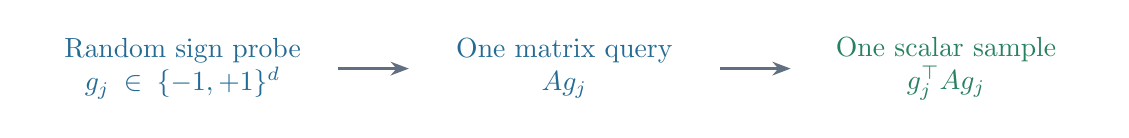
\begin{tikzpicture}[>=Stealth,every node/.style={align=center,font=\normalsize}]
\node[text=Teal,text width=3.7cm] (g) {Random sign probe\\$g_j\in\{-1,+1\}^{d}$};
\node[text=Teal,text width=3.7cm,right=.9cm of g] (ag) {One matrix query\\$Ag_j$};
\node[text=Green,text width=3.7cm,right=.9cm of ag] (x) {One scalar sample\\$g_j^\top A g_j$};
\draw[->,thick,Muted] (g.east)--(ag.west);
\draw[->,thick,Muted] (ag.east)--(x.west);
\end{tikzpicture}
\vspace{.4cm}
{\Large\[
\widehat t_s=\frac{1}{s}\sum_{j=1}^{s}g_j^\top A g_j
\]}
{\large\color{Green}\[
\mathbb E[\widehat t_s]=\operatorname{tr}(A).
\]}
\takeaway{Hutch++ uses the same averaging on a smaller residual.}
\note{The classical starting point is Hutchinson. Each probe has independent plus-or-minus-one entries. We query its matrix product, take the inner product, and obtain a scalar trace sample. The sample is unbiased, meaning its expectation is the trace. Averaging independent samples reduces variance, but each sample costs another query. Unbiasedness is not a guarantee that any one run is accurate. Hutch++ retains this random averaging but applies it to what remains after a low-rank subspace has been captured. Source: M.F. Hutchinson, Communications in Statistics--Simulation and Computation 19(2), 433--450 (1990), DOI 10.1080/03610919008812866; Meyer et al., Hutch++ Section 1.1, arXiv:2010.09649. Fixed symmetric matrix; independent Rademacher coordinates and probes.}
\end{frame}

% 3: title, citation context, method diagram, ledger, our question, page = 6.
\begin{frame}[t]{Hutch++: sketch, then sample the residual}
\context{Meyer et al.\ (2021); adaptive variants: Persson et al.\ (2022).}
\vspace{.35cm}
\centering
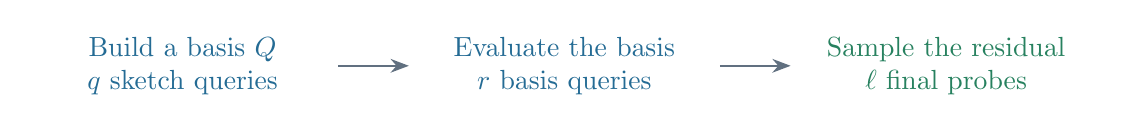
\begin{tikzpicture}[>=Stealth,every node/.style={align=center,font=\normalsize}]
\node[text=Teal,text width=3.7cm] (q) {Build a basis $Q$\\$q$ sketch queries};
\node[text=Teal,text width=3.7cm,right=.9cm of q] (r) {Evaluate the basis\\$r$ basis queries};
\node[text=Green,text width=3.7cm,right=.9cm of r] (l) {Sample the residual\\$\ell$ final probes};
\draw[->,thick,Muted] (q.east)--(r.west);
\draw[->,thick,Muted] (r.east)--(l.west);
\end{tikzpicture}
\vspace{.6cm}
{\Large\[
q+r+\ell=m,
\qquad
\underbrace{q=r=\ell=m/3}_{\text{standard full-rank split}}.
\]}
\takeaway{Our focus: reliable decisions within a fixed total budget.}
\note{Hutch++ first learns a low-rank subspace, evaluates its trace contribution, and samples the residual with Hutchinson probes. The original balanced version assigns one third of the budget to each stage. The accepted basis rank is r, which need not always equal the attempted width q. Prior adaptive variants already aim at requested accuracy, so adaptation itself is not our novelty. We study how to compare allocation choices reliably when the total budget is fixed and every query counts. Changing the sketch affects both the residual and the number of samples left for final averaging. Source: Meyer, Musco, Musco and Woodruff, SOSA 2021, arXiv:2010.09649; Persson, Cortinovis and Kressner, SIAM J. Matrix Anal. Appl. 43(3), 1162--1185 (2022), arXiv:2109.10659.}
\end{frame}

% 4: title, risk target, two requirements, uncertainty insight, page = 6.
\begin{frame}[t]{Can we trust an allocation change?}
\vspace{.2cm}
{\Large\[
\Delta
=\underbrace{\mathcal R_a}_{\text{MSE of proposed allocation}}
-\underbrace{\mathcal R_0}_{\text{MSE of baseline}}
\qquad
\text{Is }\Delta<0?
\]}
\vspace{.35cm}
\begin{itemize}\setlength{\itemsep}{.35cm}
\item Freeze both choices before gathering checking data.
\item Count construction, checking, and final sampling.
\end{itemize}
\takeaway{A lower estimated risk still needs an uncertainty argument.}
\note{Here reliable refers to trusting an allocation decision. It does not mean that Hutchinson unbiasedness is in doubt. Let R a be the final mean-squared error of a proposed allocation and R zero that of the reference baseline. The question is whether their difference is negative. We freeze the choices and their final-probe counts before drawing checking probes. We also charge construction and checking, because they reduce the final-sampling budget. A smaller estimated risk is useful evidence, but it does not automatically justify switching. We need to understand the uncertainty of that comparison. Source: integrated sections certification and confidence, particularly direct risk differences and fixed-action assumptions. Baseline risk and paid fallback must not be interchanged: returning to the baseline after spending queries cannot refund those queries.}
\end{frame}

% 5: title, observation idea, one estimator, mean insight, pairing insight, page = 6.
\begin{frame}[t]{Comparing residual risks directly}
\context{$\widehat\sigma_x^{\,2}$: residual sample variance; use the same fresh probes for both choices.}
\vspace{.35cm}
{\Large\[
\widehat\Delta
=
\frac{\widehat\sigma_a^{\,2}}{\ell_a}
-
\frac{\widehat\sigma_0^{\,2}}{\ell_0}.
\]}
\vspace{.3cm}
\bodyline{The comparison is unbiased:
$\mathbb E[\widehat\Delta]=\Delta$.}
\takeaway{Positive covariance can reduce comparison variance.}
\note{We examined the actual residual observations instead of fitting only a spectral decay model. For each frozen action, a fresh probe produces a residual quadratic form. Its sample variance estimates single-probe residual variance. Dividing by the action's own remaining final-probe count estimates its final risk. Their difference is unbiased. The same fresh probe serves both actions when their matrix products are cached and charged. Pairing can reduce the variance of the risk difference when the two risk estimates have positive covariance; sharing probes alone does not guarantee that sign. An unbiased estimate remains noisy, so this is not a confidence certificate by itself. Source: integrated certification section, exact sample-variance moments and direct common-probe risk differences, Propositions T7--T8. Independent fresh final probes are separate from the checking batch.}
\end{frame}

% 6: title, setup, analytical plot, finding, scope, page = 6.
\begin{frame}[t]{A valid bound can still be too wide}
\context{A conservative 95\% uncertainty bound for two fixed choices, given by Chebyshev.}
\centering
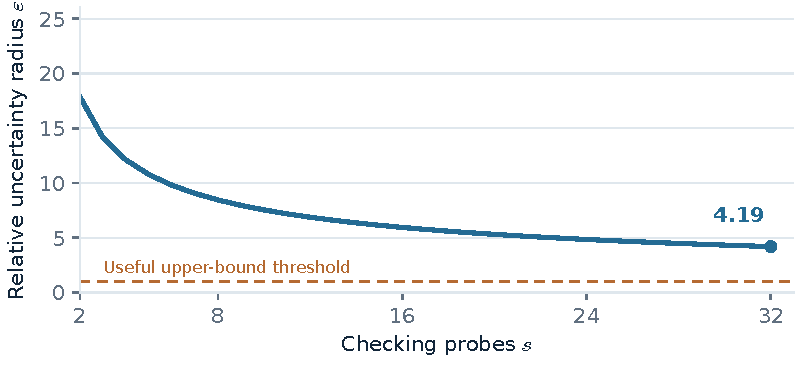
\includegraphics[width=.86\textwidth,height=3.8cm,keepaspectratio]{figures/conservative_radius.pdf}
\par\vspace{.15cm}
{\normalsize\color{Teal}\bfseries
For $2\le s\le32$, the radius exceeds 1: the bound is inconclusive.\par}
\vspace{.2cm}
{\small\color{Muted}This limits the specified bound, not every certification method.}
\note{This is a mathematical calculation, not an additional experiment. Our exact sample-variance analysis identifies the fourth-moment information needed to quantify uncertainty. The conservative degree-two envelope gives actual kurtosis at most fifteen. Combining it with Chebyshev and a two-action union bound at total failure probability five percent gives the plotted relative radius. It stays above one for checking counts two through thirty-two; even at thirty-two it is about four point one nine. Inverting this particular relative bound therefore cannot give a finite candidate variance upper bound on that grid. This does not prove that all confidence methods are impossible. The report also provides a finite paired radius under frozen nested actions and a valid pre-checking residual norm bound, but a finite radius alone does not establish useful acceptance. Source: integrated confidence section, Propositions T11 and T13. The plotted formula is epsilon squared equal to two times fourteen plus two over s-minus-one, divided by s times .05.}
\end{frame}

% 7: title, setup, real ECDF, main finding, reference, page = 6.
\begin{frame}[t]{Checking can spend away the benefit}
\context{Sample-variance heuristic: $m=160$, $s=16$; all query costs charged.}
\centering
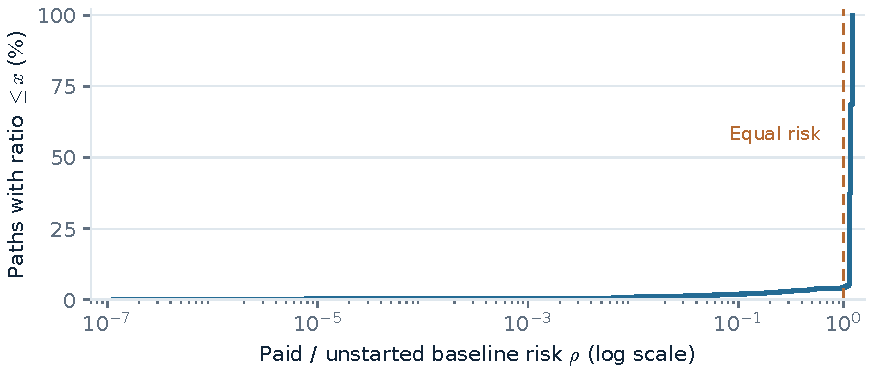
\includegraphics[width=.91\textwidth,height=3.8cm,keepaspectratio]{figures/paid_risk_ecdf.pdf}
\par\vspace{.12cm}
{\normalsize\color{Orange}\bfseries
575 of 600 paths had higher average policy risk after checking.\par}
\vspace{.18cm}
{\small\color{Muted}Can structure guide the choice before we spend on checking?}
\note{We also checked what happens when the cost of the diagnostic is included. This curve uses six hundred frozen paths from the recorded synthetic study. It evaluates the recorded sample-variance heuristic with a factor-two acceptance guard, not the conservative confidence bound on the preceding slide. No safety guarantee is attached to this empirical rule. The horizontal coordinate is average paid-policy risk divided by the original baseline risk, on a logarithmic scale. The vertical coordinate is the percentage of paths with ratio at most that value. Left of one means improvement; right of one means worse risk. Five hundred seventy-five paths, or ninety-five point eight three percent, lie above one. Each numerator averages over two hundred checking repetitions; these are not six hundred individual inaccurate trace estimates. The aggregate mean-risk summary can still improve because a small set of high-risk paths receives large protection. The result is specific to this policy and study. Source: integrated experiments E3 and figure3\_path\_source.csv. The question now is whether structure can tell us which allocations are worth considering before paying for checks.}
\end{frame}

% 8: complete content specifically requested for this revision.
\begin{frame}[t]{\fontsize{16}{19}\selectfont A smaller sketch than $m/3$ helps across many structures}
\vspace{-.08cm}
{\fontsize{10.5}{12.5}\selectfont
\begin{itemize}\setlength{\itemsep}{.04cm}\setlength{\parskip}{0pt}
\item Fixed $q\approx m/4$ vs standard $q=m/3$, same total budget
\item 186 held-out matrices, 16 groups: $\approx20\%$ lower mean normalized MSE
\item Near-optimal for power laws at tested $\eta=0.005,0.02$; fails at very small floors
\end{itemize}
}
\vspace{-.06cm}
{\fontsize{9}{11}\selectfont\color{Muted}\centering
$m=96$. Left: power law ($a=1.8$, $d=512$), cap $q\le24$. Right: held-out $q=23$ vs.\ $q=32$.\par}
\vspace{.03cm}
\centering
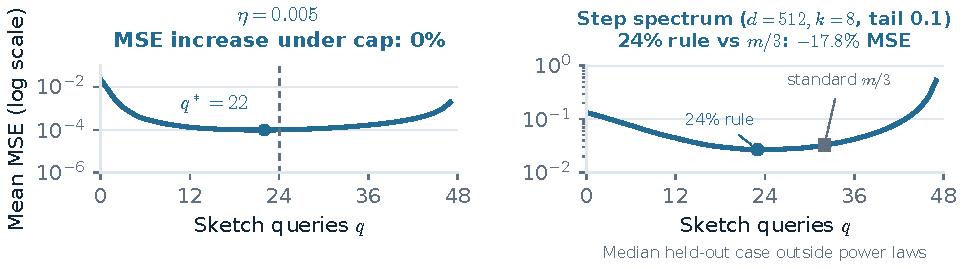
\includegraphics[width=.98\textwidth,height=3.0cm,keepaspectratio]{figures/allocation_examples.pdf}
\par\vspace{.02cm}
{\fontsize{10.5}{12.5}\selectfont\color{Teal}\bfseries
$m/3$ oversketches in many cases; how much smaller is safe\\
depends on matrix structure.\par}
\vspace{.12cm}
{\fontsize{7.1}{8.6}\selectfont\color{Muted}
Ratio chosen on training groups; $q=\lfloor0.24m+0.5\rfloor$.
A predefined 15\% rule did slightly better (22\%).\\
Means over cases; individual matrices can be hurt.\par}
\note{The top bullets retain the aggregate held-out result for the fixed twenty-four-percent rule. The left panel remains the separate offline cap test: for this power-law matrix, the observed optimum q22 lies inside the quarter cap q24. The new right panel uses a different matrix structure, chosen by a fixed median rule rather than by selecting the strongest improvement. We restricted the saved V1 curves to all 186 held-out matrices at budget 96, then excluded both power and signed-power families. This leaves 144 cases. Because that count is even, the user selected the lower-middle convention: rank 72 after sorting gains from lowest to highest, with matrix ID as a deterministic tie-break. The selected ID is 11cfff958145affe, a 512-dimensional step spectrum with head rank 8, tail 0.1 and Haar orientation. Its curve averages exact conditional MSE over 64 saved range sketches. The blue dot is the twenty-four-percent rule q23, with MSE 0.026855310105186145. The grey square is standard q32, with MSE 0.0326537944010966. The gain is 17.7574594385 percent, displayed as a 17.8 percent MSE reduction. Here the observed curve optimum is also q23, so a separate optimum marker is unnecessary. All 48 recorded widths are shown. The panels use different vertical ranges to show each full curve; compare choices within each matrix. These are existing finite-sample mean-risk estimates, not new experiments or a universal safety guarantee. Sources: V1 risk\_curves\_by\_q.csv, allocation\_policy\_comparison.csv, policy\_heldout\_summary.csv and manifest.json; the unchanged left curve uses Phase4 figure2\_actual\_and\_fixed\_basis\_risk\_curves.csv. Selection and descriptive distributions are saved separately in the source project's data folder.}
\end{frame}

% 9: title, three connected research statements, page = 5.
\begin{frame}[t]{The missing link: a cheap, reliable choice}
\vspace{.35cm}
\bodyline{\textcolor{Teal}{Recent work:} locate promising allocations.}
\vspace{.55cm}
\bodyline{\textcolor{Teal}{Earlier work:} study confidence and decision costs.}
\vspace{.55cm}
{\large\color{Orange}\bfseries
Neither gives a cheap online selection rule yet.\par}
\note{These parts address different requirements for useful adaptation. The recent experiments locate promising allocations and show how their adequacy changes with structure. The earlier analysis asks what evidence is needed to justify changing a realized allocation, and what that evidence costs. Neither result should be used as a substitute for the other. Knowing a good width exists inside a cap does not tell us which width to pick for a new matrix. Having a valid comparison bound does not show that enough improvement remains after checking. The unresolved link is an affordable decision rule using information genuinely available through matrix--vector queries. Sources: integrated report discussion; earlier certification analysis; Phase4 and V3 research conclusions. This is a synthesis of established project findings and open questions, not a new theorem or a completed estimator.}
\end{frame}

% 10: title, three takeaways, limitation, page = 6.
\begin{frame}[t]{What we learned, and what comes next}
\vspace{.15cm}
\begin{itemize}\setlength{\itemsep}{.4cm}
\item Reliable decisions need more than unbiased risk estimates.
\item Small sketches can work; the conditions depend on matrix structure.
\item Next: find cheap structural clues without spending away the benefit.
\end{itemize}
\vfill
{\small\color{Muted}
Limits: selected synthetic matrices and budgets; no universal cap or completed online selector.}
\note{The earlier work shows why reliable adaptation needs more than an unbiased risk estimate. Uncertainty and the cost of obtaining evidence both matter. The recent work shows that smaller sketches can be enough in tested regimes, but matrix structure changes which allocations are appropriate. Our immediate direction is to understand when a smaller sketch is sufficient, especially the role of spectral floor and decay. Eventually we want clues that can be obtained cheaply from a new black-box matrix, followed by a selection rule that does not spend away its own benefit. We should keep the limits explicit: most evidence is from selected synthetic matrices and budgets; no universal quarter-budget guarantee or completed online selector is established. I will stop here to leave time for questions with Swati. The preserved v10 dictionary contains the detailed mathematics and additional experiments.}
\end{frame}

\end{document}
